\documentclass[11pt]{article}

\usepackage[a4paper]{geometry}
\geometry{left=2.0cm,right=2.0cm,top=2.5cm,bottom=2.5cm}

\usepackage{ctex} % 支持中文的LaTeX宏包
\usepackage{amsmath,amsfonts,graphicx,subfigure,amssymb,bm,amsthm,mathrsfs,mathtools,breqn} % 数学公式和符号的宏包集合
\usepackage{algorithm,algorithmicx} % 算法和伪代码的宏包
\usepackage[noend]{algpseudocode} % 算法和伪代码的宏包
\usepackage{fancyhdr} % 自定义页眉页脚的宏包
\usepackage[framemethod=TikZ]{mdframed} % 创建带边框的框架的宏包
\usepackage{fontspec} % 字体设置的宏包
\usepackage{adjustbox} % 调整盒子大小的宏包
\usepackage{fontsize} % 设置字体大小的宏包
\usepackage{tikz,xcolor} % 绘制图形和使用颜色的宏包
\usepackage{multicol} % 多栏排版的宏包
\usepackage{multirow} % 表格中合并单元格的宏包
\usepackage{pdfpages} % 插入PDF文件的宏包
\RequirePackage{listings} % 在文档中插入源代码的宏包
\RequirePackage{xcolor} % 定义和使用颜色的宏包
\usepackage{wrapfig} % 文字绕排图片的宏包
\usepackage{bigstrut,multirow,rotating} % 支持在表格中使用特殊命令的宏包
\usepackage{booktabs} % 创建美观的表格的宏包
\usepackage{circuitikz} % 绘制电路图的宏包
\usepackage{caption}
\captionsetup{font=small,skip=2pt}

\definecolor{dkgreen}{rgb}{0,0.6,0}
\definecolor{gray}{rgb}{0.5,0.5,0.5}
\definecolor{mauve}{rgb}{0.58,0,0.82}
\lstset{
  frame=tb,
  aboveskip=3mm,
  belowskip=3mm,
  showstringspaces=false,
  columns=flexible,
  framerule=1pt,
  rulecolor=\color{gray!35},
  backgroundcolor=\color{gray!5},
  basicstyle={\small\ttfamily},
  numbers=none,
  numberstyle=\tiny\color{gray},
  keywordstyle=\color{blue},
  commentstyle=\color{dkgreen},
  stringstyle=\color{mauve},
  breaklines=true,
  breakatwhitespace=true,
  tabsize=3,
}

% 轻松引用, 可以用\cref{}指令直接引用, 自动加前缀. 
% 例: 图片label为fig:1
% \cref{fig:1} => Figure.1
% \ref{fig:1}  => 1
\usepackage[capitalize]{cleveref}
% \crefname{section}{Sec.}{Secs.}
\Crefname{section}{Section}{Sections}
\Crefname{table}{Table}{Tables}
\crefname{table}{Table.}{Tabs.}

\setmainfont{Palatino_Linotype}[
  Path = ../Fonts/,
  Extension = .ttf
]
\setCJKmainfont{SimHei}[
  Path = ../Fonts/,
  Extension = .ttf
]
\punctstyle{kaiming}
% 偏好的几个字体, 可以根据需要自行加入字体ttf文件并调用

\renewcommand{\emph}[1]{\begin{kaishu}#1\end{kaishu}}

%改这里可以修改实验报告表头的信息
\newcommand{\studentNum}{00000000}
\newcommand{\name}{我是谁}
\newcommand{\exDate}{2025.04.01}
\newcommand{\weekDay}{二}
\newcommand{\ap}{下午}
%%%%%%%%%%%%%%%%%%%%%%%%%%%

\begin{document}

%若需在页眉部分加入内容, 可以在这里输入
% \pagestyle{fancy}
% \lhead{\kaishu 测试}
% \chead{}
% \rhead{}

\begin{center}
    \LARGE \bf 《\, 基\, 础\, 物\, 理\, 实\, 验\, 》\, 实\, 验\, 报\, 告
\end{center}

\begin{center}
    \emph{学号}\underline{\makebox[6em][c]{\studentNum}}
    \emph{姓名}\underline{\makebox[6em][c]{\name}} 
    \emph{实验日期} \underline{\makebox[8em][c]{\exDate}}
    \emph{星期} \underline{\makebox[2em][c]{\weekDay}}\;\underline{\makebox[3em][c]{\ap}}
    {\noindent}
    \rule[8pt]{17cm}{0.2em}
\end{center}

\begin{center}
    \Large \bf 热电偶的特性及其应用
\end{center}

\section*{一、实验目的}

\begin{enumerate}
    \item 了解热电偶测温的基本原理和方法
    \item 了解热电偶定标的基本方法
    \item 掌握热电偶的基本规律
\end{enumerate}

\section*{二、实验仪器}

快速变温控温实验仪,自组装热电偶,高精度万用表,保温杯(冰块)。

\section*{三、实验原理}

\begin{wrapfigure}{r}{6cm}
    \centering
    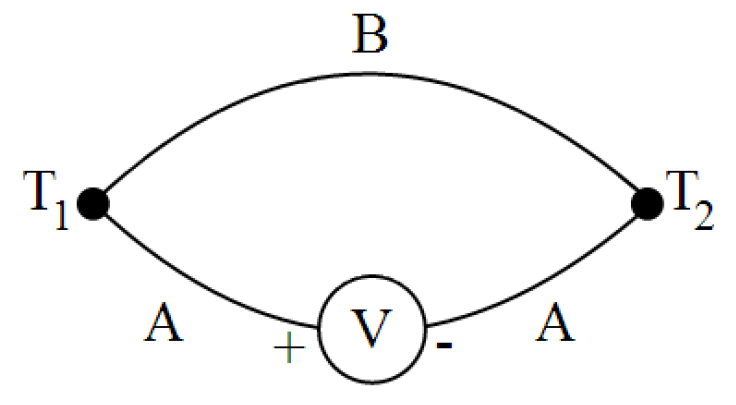
\includegraphics[width=5cm]{Figs/两种不同金属构成的闭合电路.png}
    \caption{两种不同金属构成的闭合电路}
\end{wrapfigure}

1821年塞贝克(T.\;J.\;Seebeck)发现,当构成回路的两种不同金属的两个连接点温度不同时,回路中会有恒定电流产生,这表示两种金属的接触处由于温度差而产生了电动势,即温差电动势,该现象称为塞贝克效应,这种电路称为热电偶,如图1所示。

热电偶的温差电动势与两接头之间的温度关系比较复杂,可以用下式表示:
$$
E=\int_{T1}^{T2}[S_B(T)-S_A(T)]dT
$$
$S(T)$表示金属的塞贝克系数,$T_2$为热端的温度,$T_1$为冷端的温度。但是在较小温差范围内可以近似的认为温差电动势$E$与温度差$(T_2-T_1)$成正比,即:
$$
E=C(T_2-T_1)
$$
式中$C$称为温差系数,单位为$\mu V\cdot^{\circ}C^{-1}$,它表示两接点的温度相差$1^{\circ} C$时所产生的电动势,其大小取决于组成热电偶材料的性质,即:
$$
C=\dfrac{k}{e}\cdot ln\left(\dfrac{n_{0_A}}{n_{0_B}}\right)
$$
式中$k$为玻尔兹曼常量,$e$为电子电量,$n_{0_A}$和$n_{0_B}$为两种金属单位体积内的自由电子数目。

对于热电偶而言,有如下两个常见定律:

1.\;中间导体定律
   
在热电偶回路中接入中间导体(第三导体),只要中间导体两端温度相同,中间导体的引入对热电偶回路总电势没有影响。

2.\;中间温度定律

\begin{wrapfigure}{r}{6cm}
    \centering
    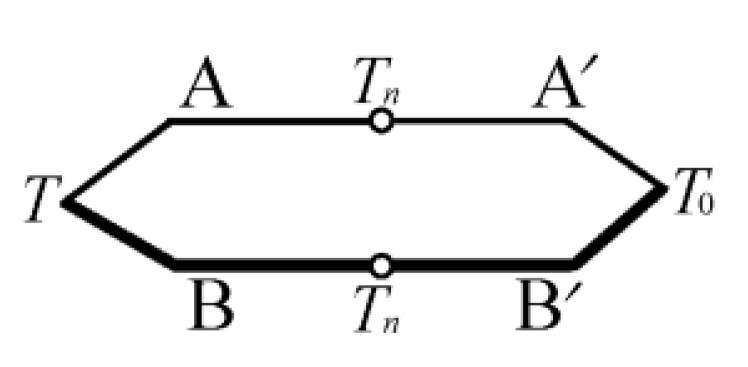
\includegraphics[width=4cm]{Figs/中间定律连线示意图.png}
    \caption{中间定律连线示意图}
\end{wrapfigure}

热电偶回路两接点(温度为$T$、$T_0$)间的热电势,等于热电偶在温度为$T$、$T_n$时的热电势与在温度为$T_n$、$T_0$时的热电势的代数和,如图2所示。$T_n$称中间温度。

\large 热电偶的定标

\normalsize
利用温差热电偶测量温度时必须进行定标,即用实验的方法测量热电偶温差
电动势与测量端温度之间的关系曲线,定标方法有以下两种:
\begin{enumerate}
    \item 比较法
    
    用被校准热电偶与一个标准热电偶或标准热电阻去测同一个温度,测得一组数据,其中被校热电偶测得的热电势即由标准热电偶或标准热电阻所测的热电势所校准,在被校准热电偶的适用范围内改变不同的温度,进行逐点校准,就可以得到被校准热电偶的一条校准曲线。这种定标方法设备简单,操作方便,但其准确程度受到标准热电偶或标准热电阻准确度的限制。
    \item 固定点法
    
    纯金属在融化和凝固过程中,其融化和凝固温度不随环境温度改变而改变,从而利用这些纯物质的融化和凝固温度作为已知温度,测出热电偶在这些温度下对应的电动势,利用作图法或最小二乘法拟合实验曲线,求出温差系数$C$,从而得到热电势与温度关系曲线。这种定标方法准确度很高,已被定为国际温标复现、校标的基准。
\end{enumerate}


\section*{四、实验内容}

本实验定标时使用快速变温控温实验仪温度(Pt100)作为参照。

\begin{enumerate}
    \item 测试实验室提供的热电偶的温差电动势随着热端温度变化的特性
    
    测试时。保持冷端处于$0^{\circ} C$(冰水混合物),热端温度从$30^{\circ} C$到$70^{\circ} C$之间每变化$5^{\circ} C$记录一次温控电动势的值。根据测得数据作图$E-T$,求出温差系数$C_1$。

    \item 验证中间导体定律
    
    将第三种金属串联接入上述热电偶电路中,并使第三种金属的两个连接端处于相同的温度,测试该热电偶的温差电动势随着热端温度的变化特性。根据测得数据作图$E-T$,求出温差系数$C_2$。比较步骤1和步骤2所得数据,比较$C_1$和$C_2$,验证中间导体定律。
    \item 验证中间温度定律
    
    以人体手温(约为$35^{\circ} C$)作为中间温度,保持冷端处于$0^{\circ} C$,手握热端,测得$E_{0-\text{手}}$;保持热端处于$75^{\circ} C$,手握冷端,测得$E_{\text{手}-75}$;保持冷端处于$0^{\circ} C$,热端处于$75^{\circ} C$,测得$E_{0-75}$,验证中间温度定律。
\end{enumerate}

\section*{五、数据记录}

原始数据详见附页。

\section*{六、数据处理}

\begin{enumerate}
    \item 测量热电偶系数
    根据数据绘制$E-T$曲线(见图3),根据拟合曲线得到的斜率,得出热电偶的温差系数$C_1=63.47\pm0.13\;\mu V^{\circ}C^{-1}$。
    
    \begin{figure}[H]
        \centering
        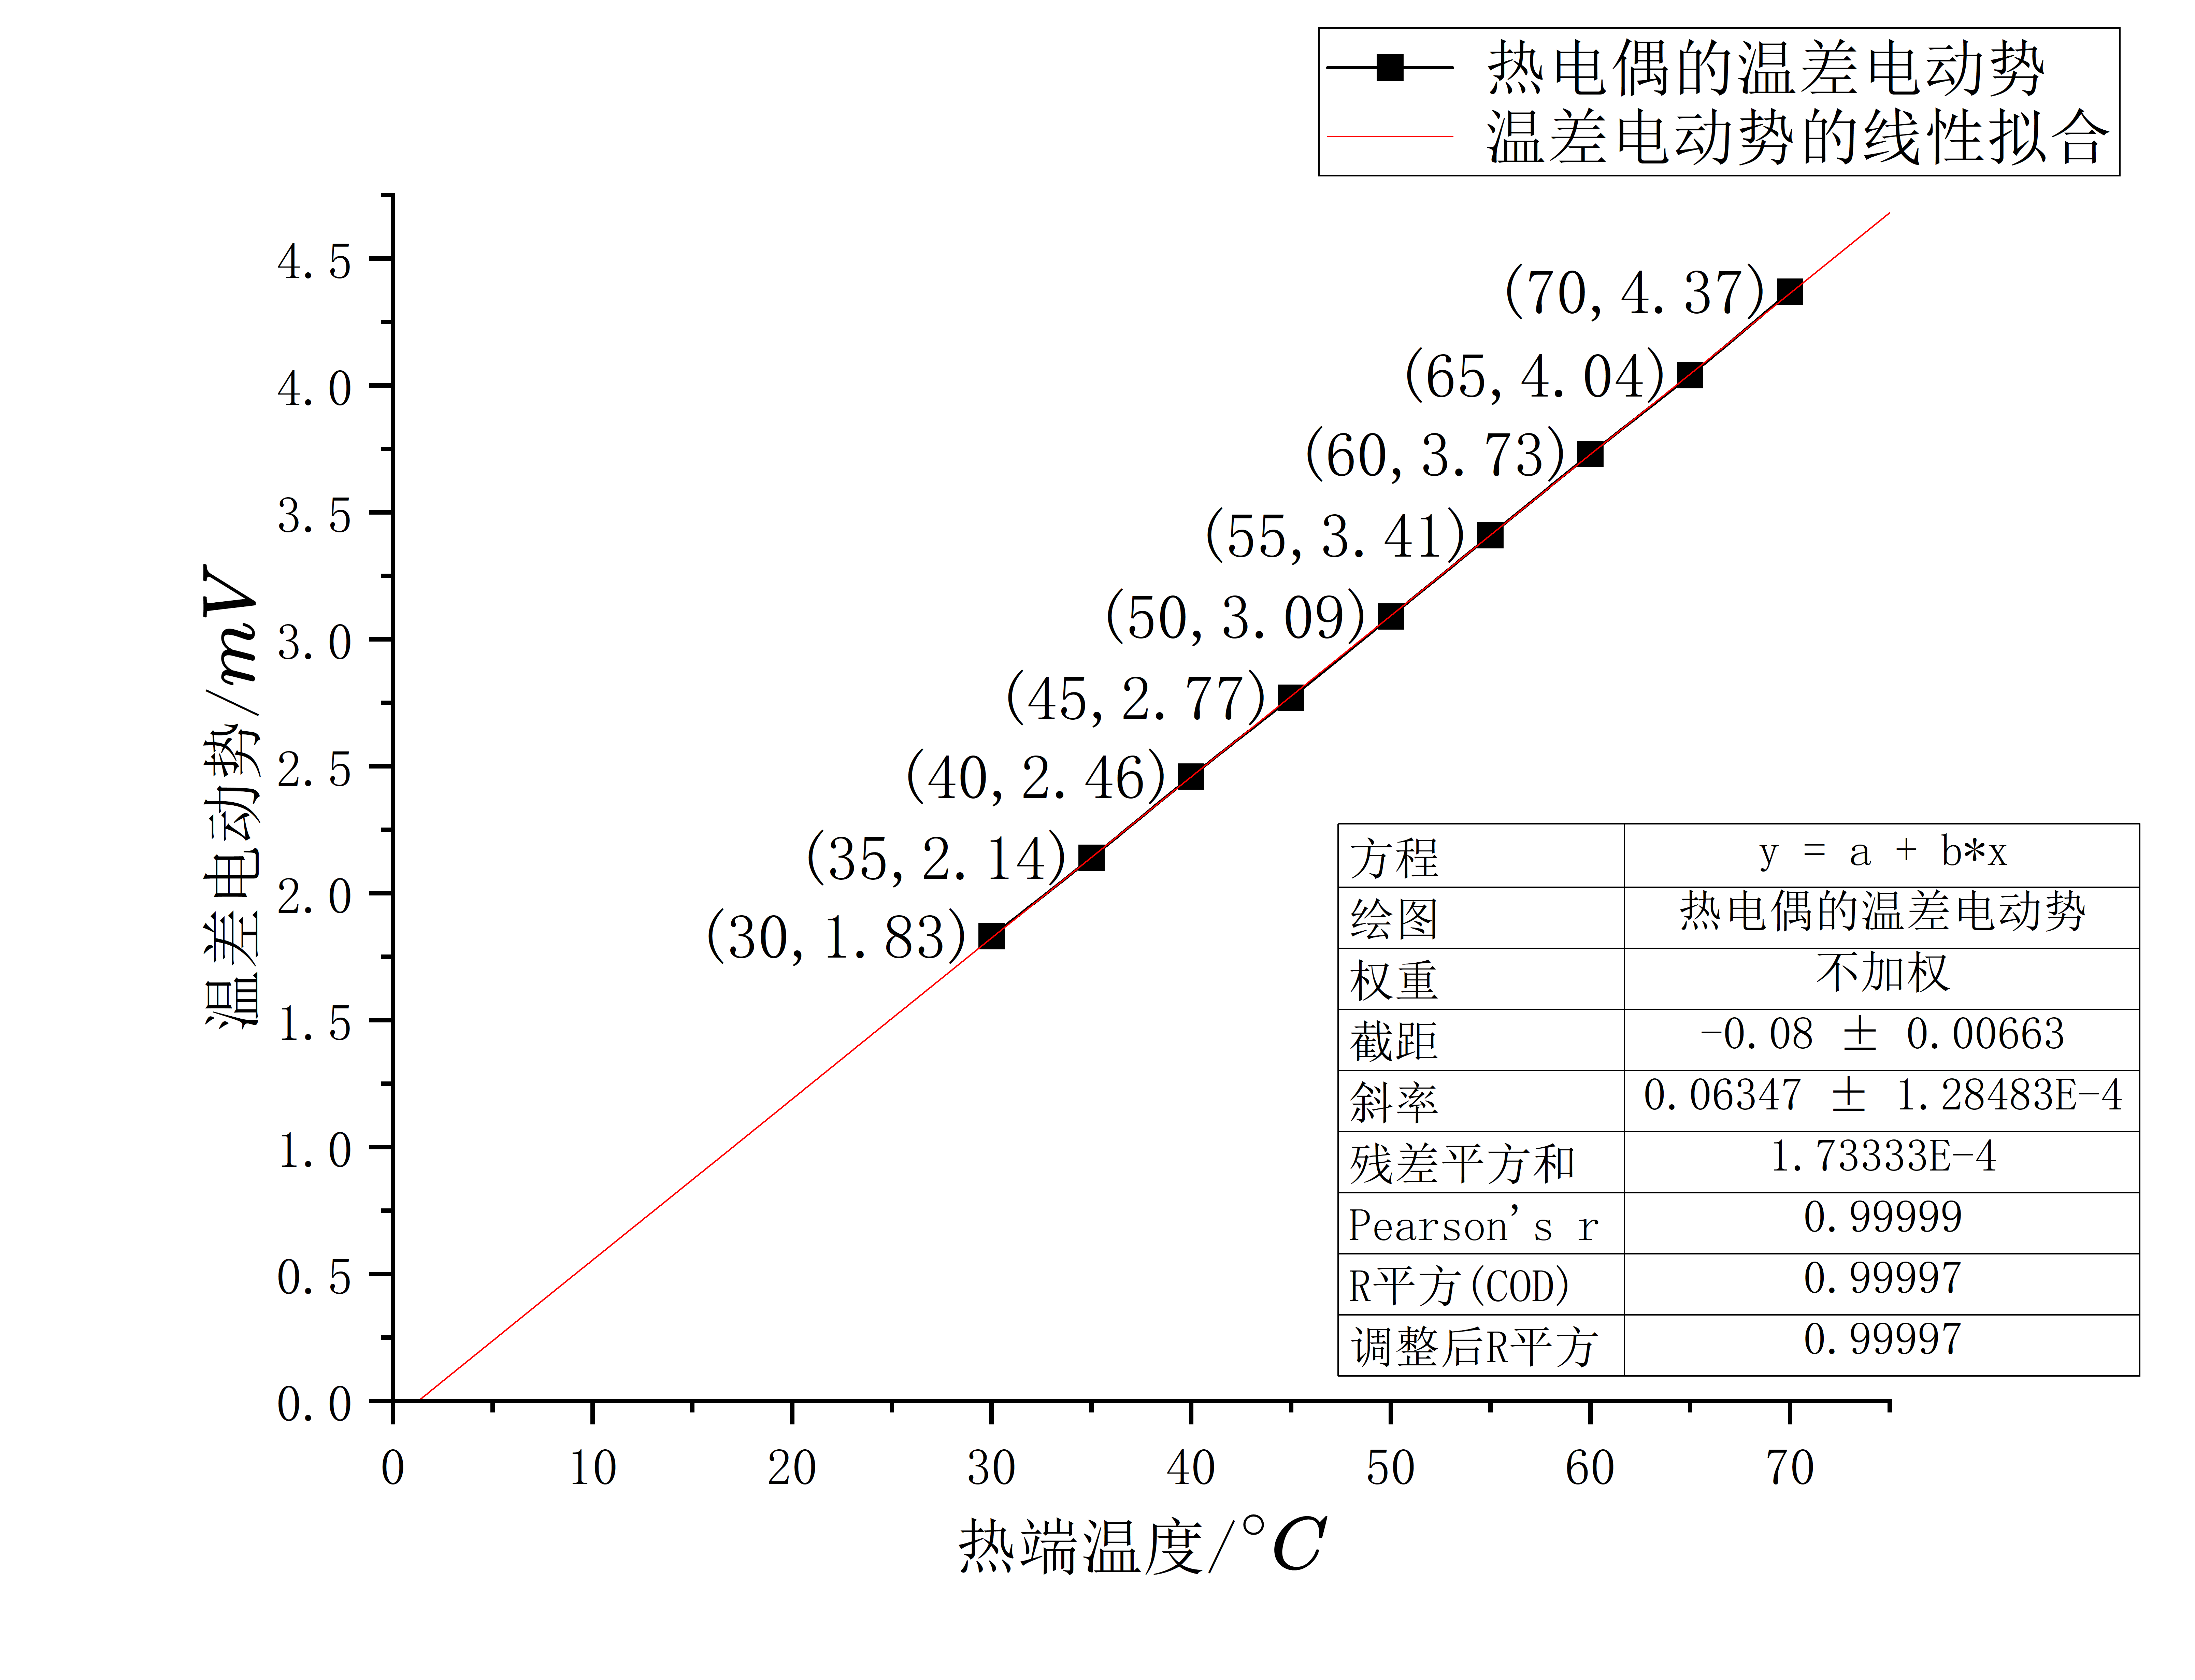
\includegraphics[width=13.5cm]{Figs/Graph1.png}
        \caption{\normalsize 热电偶的$E-T$曲线及其线性拟合}
    \end{figure}

    \item 验证中间导体定律
    
    根据数据绘制$E-T$曲线(见图4),根据拟合曲线得到的斜率,得出热电偶的温差系数$C_2=64.03\pm0.19\;\mu V^{\circ}C^{-1}$。比较$C_1$和$C_2$,$C_1\approx C_2$,得以验证中间导体定律。
    
    \begin{figure}[H]
        \centering
        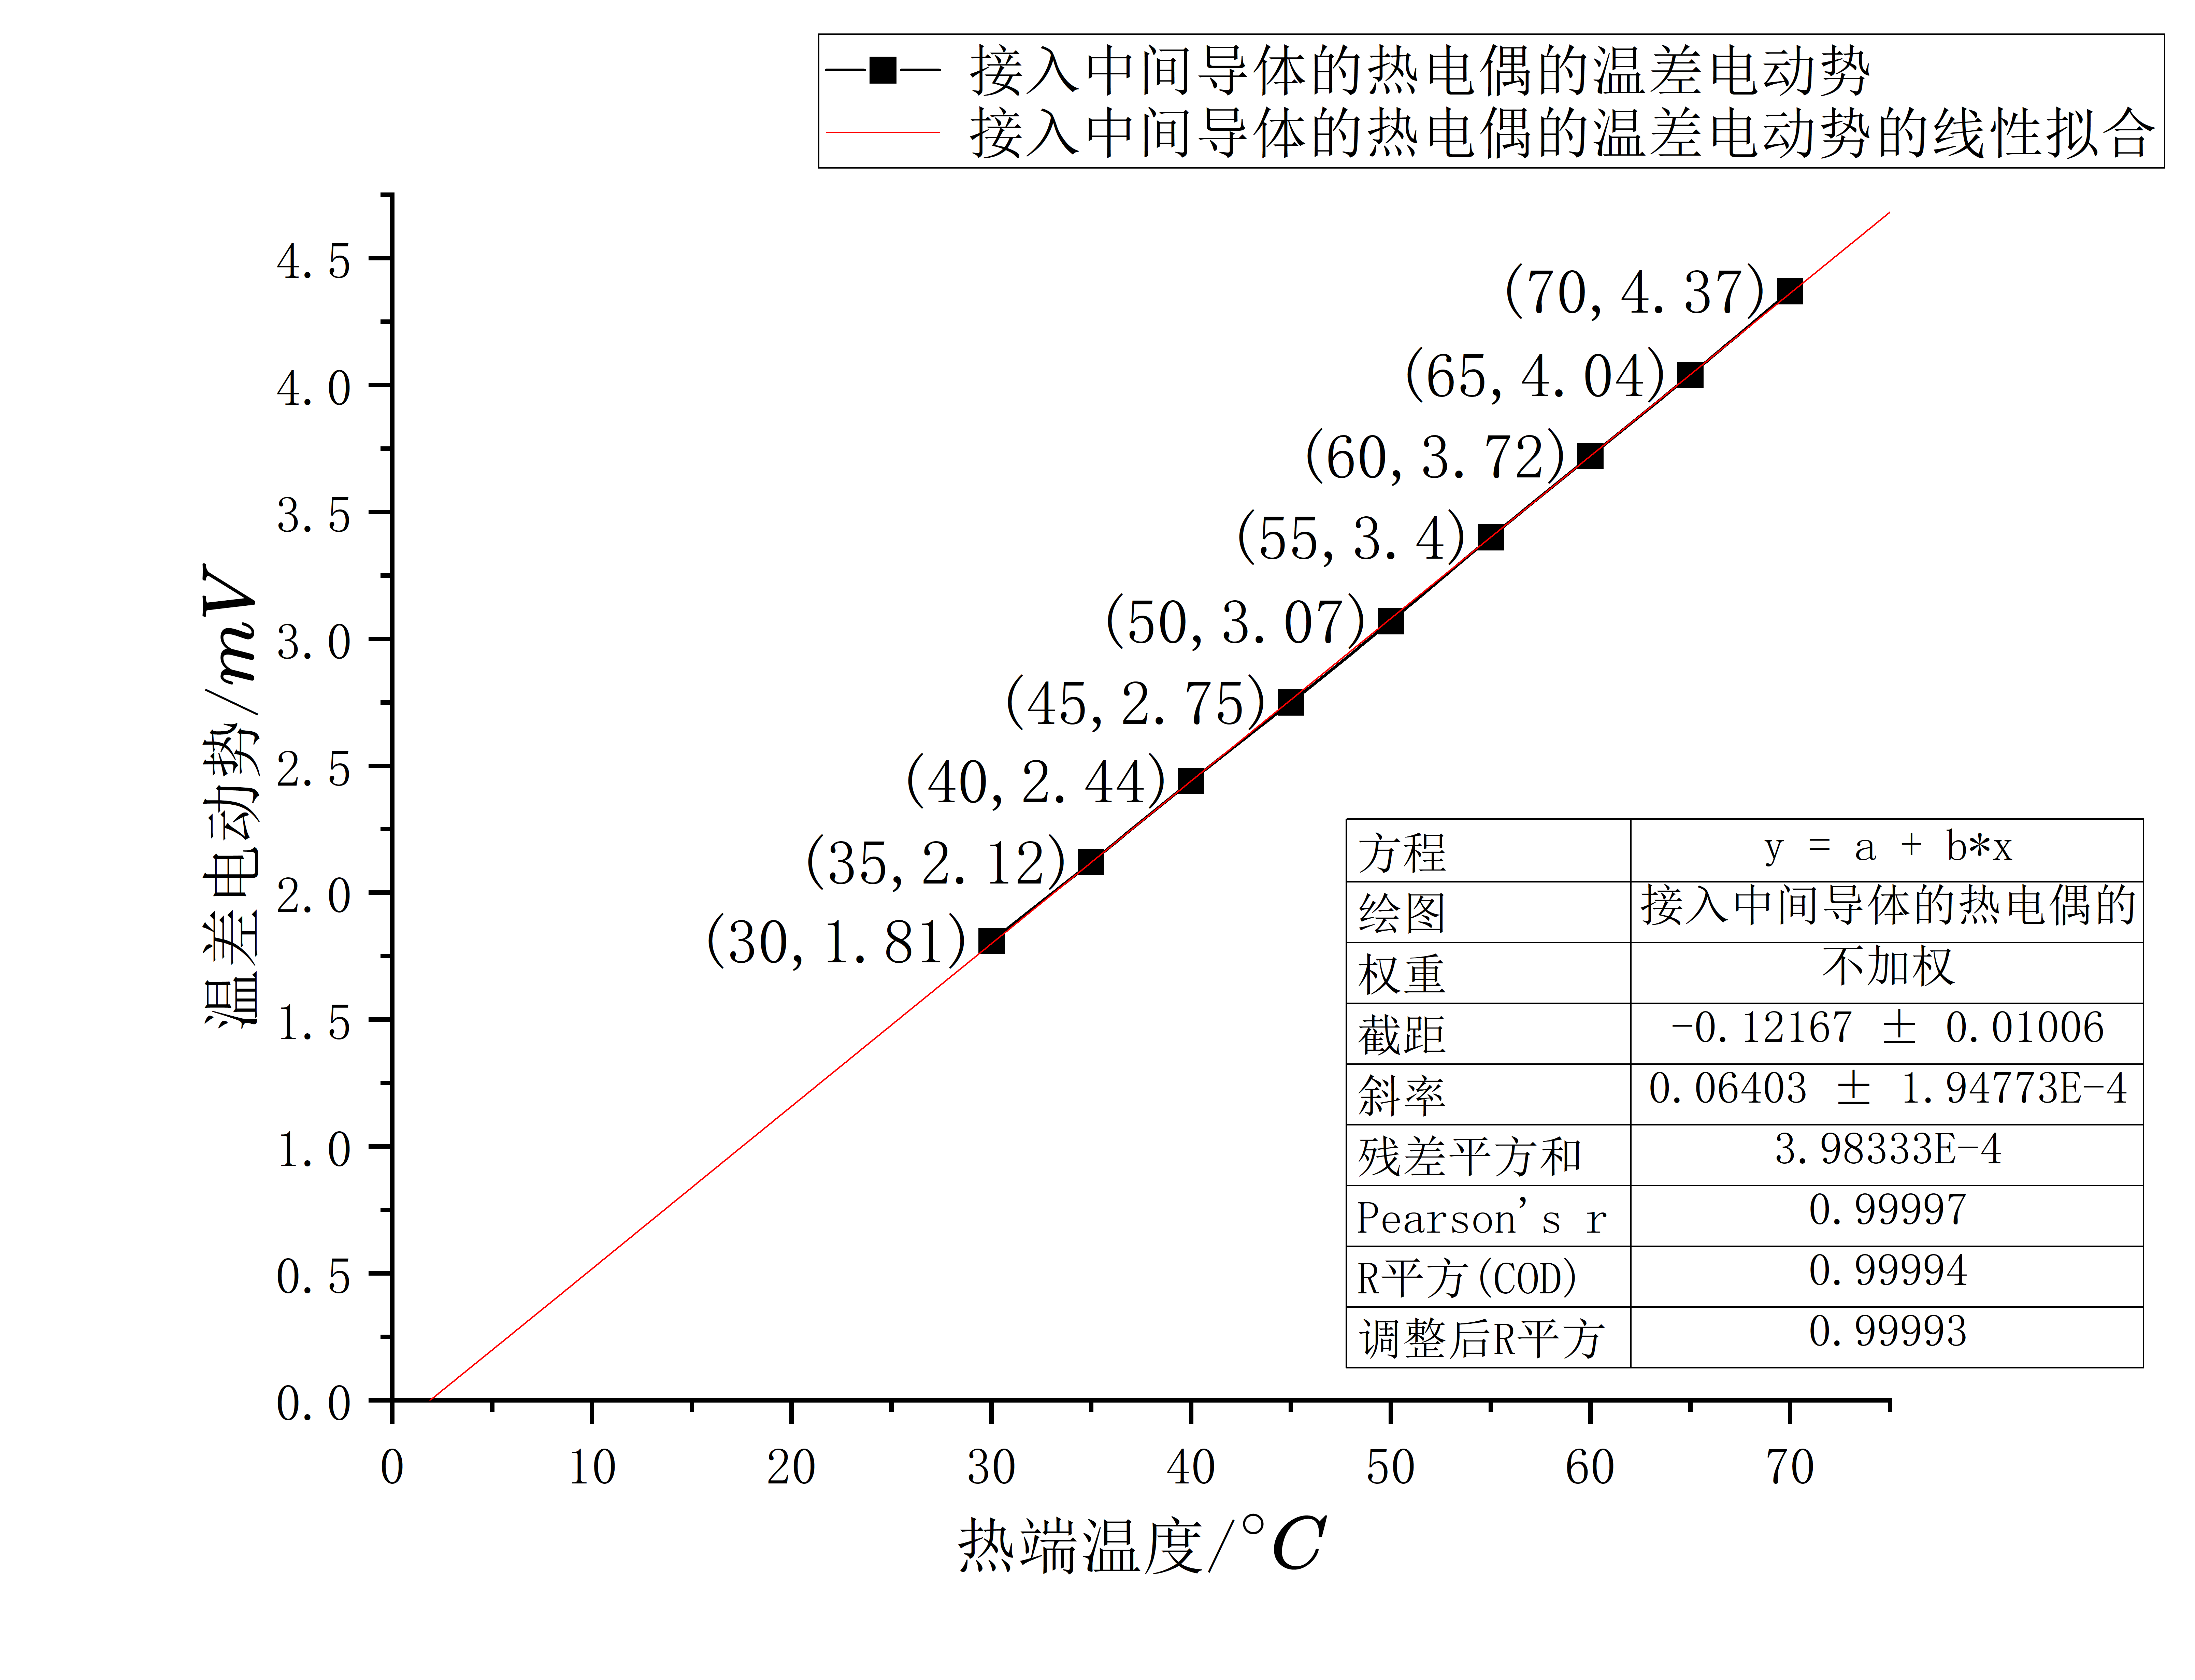
\includegraphics[width=13.5cm]{Figs/Graph2.png}
        \caption{\normalsize 接入中间导体的热电偶的$E-T$曲线及其线性拟合}
    \end{figure}

    \item 验证中间温度定律
    
    根据数据可知,$E_{0-\text{手}}=2.02\;mV;\;E_{\text{手}-75}=2.59\;mV$,则$E_{0-\text{手}}+E_{\text{手}-75}=4.61mV;\;E_{0-75}=4.69\;mV$,相对误差为$u=\dfrac{|(E_{0-\text{手}}+E_{\text{手}-75})-E_{0-75}|}{E_{0-75}}\times100\%=1.706\%$,可以近似认为$E_{0-\text{手}}+E_{\text{手}-75}\approx E_{0-75}$,得以验证中间温度定律。

\end{enumerate}

\section*{七、误差分析}

\begin{enumerate}
    \item 实验室中有大量会发射电磁波的设备,会对高精度电压表的测量造成干扰,导致测量结果不准确。
    \item 恒温箱的温度呈现阻尼振动,需要较长时间稳定,且难以达到完全稳定。
    \item 热端温度会受到室温的影响,冷端的温度会受到保温杯内壁的影响,导致温度不稳定。
    \item 接入的中间导体的两端温度不完全相同,可能会导致中间导体定律的验证不完全准确。
    \item 手捏住热端/冷端时,手的温度不稳定,可能会导致中间温度定律的验证不完全准确。
\end{enumerate}

\section*{八、思考题}

在温度相关的实验中,常采用先升温后降温再取平均值的方法,该方法的优点是什么?该方法是否也适用于本实验?为什么?
\\答:

\begin{enumerate}
    \item 减少热滞效应的影响;
    
    许多温度传感器或被测系统存在热惯性,导致升温与降温过程中温度变化的响应速度不一致。通过双向测量并取平均,可以部分抵消这种动态误差,提高数据的准确性。
    \item 平衡系统误差;
    
    实验装置的热膨胀、环境温度波动等因素可能导致升、降温时的测量值存在方向性偏差。取平均值有助于平衡此类系统性误差,使结果更接近真实值。
    \item 识别材料特性差异。
    
    某些材料的物理性质在升、降温过程中可能不同。双向测量能更全面地反映材料特性,而取平均可简化复杂行为的分析。
\end{enumerate}

适用于热电偶特性测试和中间导体定律的验证,但不适用于中间温度定律的验证。

因为中间导体定律的验证是基于热电偶在不同温度下的电动势关系,升、降温时的测量值可能会受到热滞效应的影响,导致结果不准确。通过升、降温两次测量并取平均值,可有效抵消热滞引起的系统误差。中间温度定律验证无动态温度变化需求,只需在特定温度下测量电动势,因此不需要升、降温两次测量并取平均值。

\section*{九、实验结论}

本实验使用快速变温控温实验仪(Pt100)的温度为参照,测量了热电偶的温差电动势随着热端温度变化的特性,并通过统计学方式得到了其温差系数$C_1=63.47\pm0.13\;\mu V^{\circ}C^{-1};\;C_2=64.03\pm0.19\;\mu V^{\circ}C^{-1}$,得出接入中间导体前后的温差系数$C_1\approx C_2$,验证了中间导体定律,通过测得$E_{0-\text{手}}=2.02\;mV;\;E_{\text{手}-75}=2.59\;mV;\;E_{0-75}=4.69\;mV$,故而$E_{0-\text{手}}+E_{\text{手}-75}\approx E_{0-75}$,验证中间温度定律。实验结果表明,热电偶的温差电动势与温度差成正比,且中间导体定律和中间温度定律均成立。

\end{document}